\clearpage
\section{Physical Deployment Pilot}\label{physical-deployment}
The physical deployment is a declared joint-exploration variant, distinct from the supplied-graph, two-template controlled study. It uses exploration\_joint\_v1 derived from v10\_3\_1, with revised joint unknown-coverage and measured-surface candidate generation, real-scene semantics, measured sensor-range and 3 m extent adapters (rather than the original 2.2 m applicability cap), default CSM keyframes, measured CAN controller velocity and fixed SE2 alignment. The camera had been relocated without recalibrating its earlier extrinsics; its earlier self-mask was disabled. The navigation map retained prior observations in the first episode.

One S40 episode completed 40 paid actions and 40 arrivals, returned to its grid anchor, and acquired 41 frames over 7.394 m of CAN-estimated travel and 542.444 s. Its observed-area proxy increased from 72.08 to 128.28 m$^2$, while its fixed old-surface quality proxy decreased from 0.213760 to 0.199107. These are internal proxies, without an independent map or surface-accuracy reference. All 12 recorded planning states gave equal G and S scores for shared candidates; only two had multiple candidates. This does not constitute a separate G trial.

\subsection{Fresh-map ordered C/S physical pilot}

A subsequent pilot executed coverage-only C followed by joint S in the same physical scene. Each arm used a fresh, separately supervised stock gmapping instance and a new policy session, with the same 40-action budget, 600 s limit, circular footprint, candidates, return rule, sensing configuration and execution protection. Only score mode differed within the policy configuration; C retained the same candidate generator and sensor modalities. CSM odometry and the display TSDF remained continuous. The actual bootstraps differed by 0.0701 m and 0.0672 rad, and their initial navigation-known masks differed in 205 cells (8.20 m$^2$) on the common 0.2 m planning grid. This is an approximate starting-condition comparison, not identical-input pairing.

\begin{table}[!htbp]
\caption{One ordered physical C/S pilot with fresh navigation maps; failures remain included}\label{tab:physical-pair}
\small\renewcommand{\arraystretch}{1.12}\setlength{\tabcolsep}{3pt}
\begin{tabular}{@{}>{\raggedright\arraybackslash}p{.18\linewidth}p{.12\linewidth}p{.18\linewidth}p{.17\linewidth}p{.23\linewidth}@{}}
\toprule
Arm and termination & Paid / obs. & CAN / time & Internal area (m$^2$) & Own-support old-quality \\
\midrule
C: budget exhausted, returned & 40 / 41 & 6.741 m /\newline 558.214 s & 66.40 $\to$ 123.44 & 0.249536 $\to$ 0.190989 (270 points) \\
S: method failure, no return & 32 / 33 & 5.233 m /\newline 451.992 s & 65.32 $\to$ 122.00 & 0.234949 $\to$ 0.299275 (290 points) \\
\bottomrule
\end{tabular}
\end{table}



\begin{figure}[!htbp]
\centering
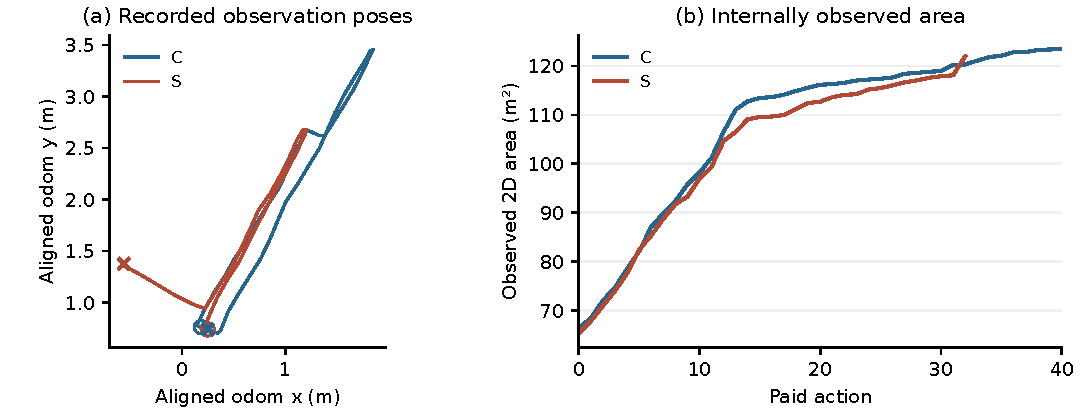
\includegraphics[width=\linewidth]{PhysicalPair_C_S_20261107.pdf}
\caption{Recorded aligned-odometry poses and internal observed-area proxy in the ordered C/S pilot. S stops after action 32; no continuation is inferred. The two episodes use different initial measurements and provide no independent accuracy reference.}
\label{fig:physical-pair}
\end{figure}

C completed its budget and returned to the discrete anchor. S stopped after its 32nd accepted action when the existing circular-footprint check reported \texttt{current\_footprint\_not\_known\_safe}; it did not return. This was an original method check, not a newly introduced policy gate. CAN feedback was zero after both runs. Unequal completed actions, the failed S return, and different initial information prevent an efficiency ranking or a causal policy-benefit claim. Quality is reported separately on each arm's own fixed bootstrap support, whose identities differ; the C decrease and S increase are not a matched reconstruction-accuracy comparison. This C/S objective ablation does not isolate a semantic S/G effect.

At paid action 12, both runs replanned after the original next-footprint check; at each run's own state, C and S selected the same candidate, while the maps differed across runs. At S action 31, frozen-state C had no positive candidate whereas G and S selected the same positive candidate. These recorded counterfactuals are not additional physical trials, and G/S ties do not establish a semantic decision effect.

A mapper-only replay of the retained S observations reproduced the final belief: a measured 0.504 m laser return inserted a nearby occupied cell before depth fusion, while the input navigation grid alone still passed the footprint check. This identifies the recorded fusion source, not the physical object or a verified noise or localization cause.


% Single insertion point for new physical evidence. Replace only from verified terminal records.
\subsection{Calibrated 24-action integration run}

After revising the camera extrinsics, a later S24 integration episode completed 24 paid actions, 24 verified arrivals and 25 observations, returning to its discrete anchor over 3.591 m of CAN-estimated travel and 368.847 s. This episode used a different sensor calibration and map state from the earlier C/S pilot and is not a matched continuation or policy comparison. All six newly recorded planning states gave equal G/S candidate scores and zero incremental aperture contribution, so they show no semantic selection effect.

After the run, the operator reported that localization had drifted during the preceding manual relocation to the test area. The drift onset was not established, so the map at S24 initialization may already have been affected. Discrete-anchor acceptance and measured travel therefore support bounded execution integration, not independent localization accuracy, comparative exploration efficiency or reconstruction accuracy. The internal area proxy (180.12 to 256.60 m$^2$) is not treated as verified newly discovered physical area. A subsequent mapping reset starts a new epoch; its observations cannot be pooled with this episode as a shared initial map.

\subsection{Calibrated fresh-map C/S comparison}

A new ordered C/S pilot used independently restarted stock gmapping maps and fresh acquired initial packets in the reset localization epoch. Both arms retained the same 40-action allowance, 600 s external limit, circular footprint, candidate generator, return rules, sensor configuration and ROS/hardware protection. The score mode was the policy difference; this remains a coverage-only versus joint-objective comparison, not a semantic-only ablation. The planning transform was identical and anchored at the actual C start. Initial odometry differed by 0.06695 m and $-0.06259$ rad, while the initial navigation-known masks differed in 430 cells (17.20 m$^2$) on the common grid. Similar initial area therefore does not imply identical initial information.

\begin{table}[!htbp]
\caption{One further ordered C/S pilot after calibration and map reset. Both arms have a 40-action/600 s allowance; actual exposure and return differ. Internal quality uses a separate fixed bootstrap support in each arm.}\label{tab:physical-pair-calibrated}
\small\renewcommand{\arraystretch}{1.12}\setlength{\tabcolsep}{3pt}
\begin{tabular}{@{}>{\raggedright\arraybackslash}p{.18\linewidth}p{.12\linewidth}p{.18\linewidth}p{.17\linewidth}p{.23\linewidth}@{}}
\toprule
Arm and termination & Paid / obs. & CAN / time & Internal area (m$^2$) & Own-support old-quality \\
\midrule
C: no positive option at anchor, returned & 24 / 25 & 3.738 m /\newline 342.345 s & 65.24 $\to$ 98.52 & 0.165048 $\to$ 0.277736 (479 points) \\
S: anchor-footprint failure, no return & 13 / 14 & 1.857 m /\newline 184.862 s & 65.32 $\to$ 88.88 & 0.193484 $\to$ 0.180111 (437 points) \\
\bottomrule
\end{tabular}
\end{table}

C completed 24 verified arrivals and stopped normally under the original rule that stops when no positive option remains at the anchor. S completed 13 verified arrivals, then failed the original check requiring the anchor footprint to remain known safe without returning. Neither endpoint was an external timeout or interruption, and both recorded zero CAN feedback after closing. At S action 10, the original next-footprint rejection triggered replanning; C and S would select different candidates at that saved state, while G and S were tied. Across both episodes, all five candidate-bearing planning states gave equal G/S scores; the terminal S state had no candidates. These are within-state diagnostics, not separately executed alternatives.

The shorter failed S route supplies no efficiency benefit. Unequal completed exposure, different initial measurements and distinct fixed surface supports prevent a matched endpoint-quality or causal policy ranking. This is one ordered pair in one physical scene, with no independent localization, map or surface-accuracy reference. No return override or replacement policy was introduced after the anchor check failed.

\subsection{Unknown-space exploration with recorded execution failures}

Further real-robot episodes extended unknown-space observation under the same declared exploration\_joint\_v1 decision policy and circular footprint. These episodes retained the real\_scene\_structural\_v1 category mapping, 4 m depth/8 m laser range profile and measured\_extent\_3m\_v1 geometry adapter. The camera transform used the confirmed relocated mount; its height reference reused the frozen depth-ground calibration scalar. A native snapshot handoff changed the execution synchronization, and the camera used SDK confidence/texture thresholds of 50/100. These input and execution adaptations remain separate from the controlled two-template study. Each episode has its own measured initial state; the records do not form a matched policy comparison.

\begin{table}[!htbp]
\caption{Additional physical S-mode episodes. Paid actions, accepted observations and verified ROS primitive arrivals are separate counts. Return denotes recorded discrete-anchor acceptance. Laser union uses only archived scans; a dash denotes an unevaluated quantity. Each row is a separate episode; interrupted attempts remain included.}\label{tab:physical-latest}
\small\renewcommand{\arraystretch}{1.13}\setlength{\tabcolsep}{3pt}
\begin{tabular}{@{}>{\raggedright\arraybackslash}p{.25\linewidth}p{.14\linewidth}p{.11\linewidth}p{.15\linewidth}p{.15\linewidth}p{.10\linewidth}@{}}
\toprule
Episode / outcome & Paid / obs. / arrivals & CAN (m) & Time (s) & Laser union (m$^2$) & Return \\
\midrule
10 Nov., S40: budget exhausted & 40 / 41 / 40 & 6.757 & 440.471 & 73.68 $\to$ 108.00 & Yes \\
12 Nov., S96: speed-stop interruption & 60 / 61 / 60 & 11.082 & 652.884 & 61.72 $\to$ 117.92 & No \\
12 Nov., 0.05 m/s S12: budget exhausted & 12 / 13 / 12 & 0.999 & 152.767 & --- & Yes \\
12 Nov., 0.05 m/s S40: speed-stop interruption & 9 / 10 / 9 & 1.484 & 136.336 & 49.76 $\to$ 62.92 & No \\
\bottomrule
\end{tabular}
\end{table}

The 10 November S40 episode completed its allowance and returned. The 12 November S96 episode acquired 61 accepted observations and completed 60 verified primitive arrivals before a CAN velocity sample of 0.154 m/s exceeded the unchanged 0.15 m/s stop threshold during the next goal. The run stopped with zero feedback and did not return; its partial coverage is retained as an interrupted outcome. In the S96 episode, the original next-footprint check rejected the outbound option at paid actions 29 and 56, triggering replanning on the latest measured map before either selected endpoint was reached. The initial coverage option forecast unknown laser and camera support, and the later route remained subject to the original return-budget check.

\begin{figure}[!htbp]
\centering
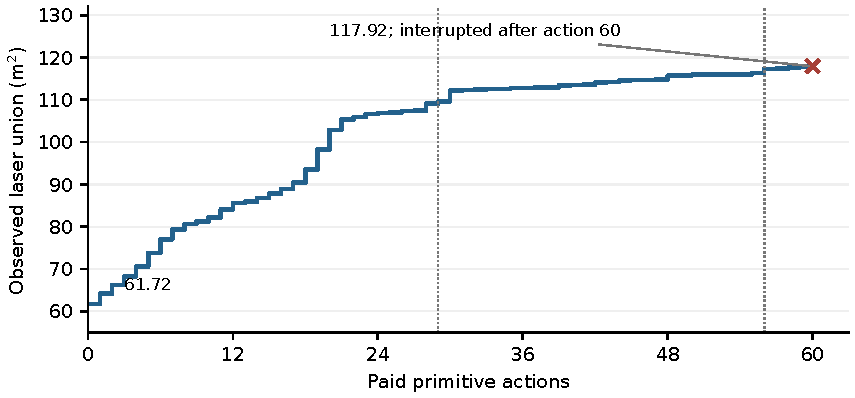
\includegraphics[width=.84\linewidth]{Physical_S96_20261112.pdf}
\caption{One interrupted physical S96 trajectory. The cumulative observed laser union increases from 61.72 to 117.92 m$^2$ across 61 saved scans, one per accepted RGB-D observation. Dotted lines mark recorded next-footprint replans at actions 29 and 56. The cross marks the last accepted observation at action 60; the subsequent goal was interrupted by the CAN speed stop. Rasterization uses a 0.2 m grid, an 8 m measured-range cap and a fixed 12.5 m-radius measurement region. The curve measures acquired ray/endpoint evidence in estimated poses, without a known traversable-area denominator or independent map reference. Checkpoints belong to one trajectory.}\label{fig:physical-S96}
\end{figure}

For these two episodes, saved-scan evaluation accumulates the union of measured laser ray and endpoint cells within the fixed region. Nonfinite or invalid returns are skipped; returns clipped at 8 m provide free-ray evidence without a hit endpoint. Only one archived scan per accepted RGB-D packet enters the curve. The resulting increases of 34.32 and 56.20 m$^2$ quantify additional recorded observation support. Pose error, coarse cells and free/hit conflicts prevent interpreting this quantity as independently verified free space or a coverage percentage. The fixed-bootstrap surface-quality proxy increases from 0.196912 to 0.348033 in S40, whereas S96 decreases from 0.224206 to 0.223401; neither is reconstruction accuracy.

All three candidate-bearing global decisions in each episode give identical G/S scores and zero incremental aperture contribution. S96 already has class-3 semantic points at initialization, but all recorded asset-entry roles report no unused feasible aperture pose; deep roles require an available entry. At its two later global decisions, none of the current geometry assets has marked semantic support despite class-3 points elsewhere in the accumulated ledger. The observed semantic frontend therefore does not demonstrate a semantic selection benefit. These saved-state G scores are diagnostics within the executed S route, not separately executed geometric-control trajectories.

A separately declared execution profile capped positive adapter commands at 0.05 m/s while preserving the decision policy, CAN stops, expiry limits and authorized correction reverse bound of $-0.05$ m/s. Its S12 episode returned after 12 arrivals, but a subsequent S40 attempt stopped after nine arrivals on the same 0.15 m/s feedback check and did not return. The passive CAN observer recorded command frames no greater than 0.05 m/s and peak velocity feedback of 0.159 m/s during that attempt. This measurement does not independently establish command acceptance or physical speed; it shows that the command cap did not prevent the recorded feedback fault. Both episodes stopped with zero feedback. Their own-support quality changes were $-0.006951$ and $-0.000236$. The short completion therefore establishes neither a resolved execution fault nor improved exploration efficiency.


